\documentclass{article}
\usepackage[czech]{babel}
\usepackage[utf8]{inputenc}
\usepackage[T1]{fontenc}
\usepackage{indentfirst}
\usepackage{hyperref}
\usepackage{graphicx}
\usepackage{caption}
\usepackage{subcaption}

\graphicspath{ {/home/shanigen/Pictures/} }

\setcounter{tocdepth}{4}
\setcounter{secnumdepth}{4}

\title{Profilování CPU implementace KCF trackeru}
\author{Karafiát Vít}

\begin{document}
\pagenumbering{gobble}
\maketitle
\newpage
\tableofcontents
\newpage
\pagenumbering{arabic}
	
\section{Úvod}
Tento dokumnet obsahuje výsldky profilování KCF trackeru ( \url{https://github.com/vojirt/kcf} ). K profilování byly použity následující programy:
\begin{itemize}
	\item Perf
	\item Hotspot \url{https://github.com/KDAB/hotspot}
	\item Intel® VTune™ Amplifier XE for Linux
	\item Valgrind-massif
	\item Massif-visualizer
\end{itemize}

\section{Postup}
Při profilování byl použit datasety z VOT 2016 pod jménem bag,ball1 a car2.\url{http://data.votchallenge.net/vot2016/vot2016.zip}\\
Profilování proběhlo na notebooku ThinkPad x220 s Intel(R) Core(TM) i7-2620M CPU @ 2.70GHz a 8GB RAM.

\subsection{Perf+Hotspot}
\label{Perf}
První použítý program na profilování byl linuxový program Perf spolu s programem Hotspot, který umožňuje vizualizaci výsledku z Perfu.\\
\newline
\textbf{Použitý příkaz:} perf record --call-graph dwarf -e r534f2e,r53412e ./kcf\_vot\\\\
R534f2e a r53412e jsou raw hardware event descriptory (Hardware eventy specifické pro danou architekturu CPU.). Kde r534f2e jsou LLC(Last Level Cache)\_REFERENCES a r53421e jsou LLC\_MISSES pro Intel Sandy Bridge. K zjistění kódů byl použit libpfm4 \url{https://sourceforge.net/p/perfmon2/libpfm4/ci/master/tree/}.

\subsection{Intel® VTune™ Amplifier XE 2017 Update 4 for Linux}

Druhý použítý program byl placený profilovací program od Intelu. VTune™ Amplifier (dále jen Amplifier) umožňuje přístup ke všem performance counterum (Speciální registry na mikroprocesorech sloužící k ukládání hardwerových aktivit v počítačových systémech.) bez potřeby je vyhledávat v manuálu k danému procesoru a automaticky udělá i vizualizaci výsledků. Použitá byla analýza na změření LLC-Hit a LLC-Miss.

%\subsection{Valgrind-massif+Massif-visualizer}
%Poslední použítý profilovací program je Massif, který je součástí Valgrindu. V nahodných momentech v průběhu programu ukazuje vzhled heapy programu. Dohromady s ním byl použít Massif-Visualizer,který umožňuje výsledek Massifu převést do grafu s časovou osou.\\
%\newline
%\textbf{Použitý příkaz:} valgrind --tool=massif
%./kcf\_vot

\section{Popis programu}
Program je implementace algorimtu z "High-Speed Tracking with Kernelized Correlation Filters" v C++ \url{http://arxiv.org/abs/1404.7584}. Víc informací o programu je k dispozici na \url{https://github.com/vojirt/kcf}\\
Trax část KCF trackeru nebyla použita.
\subsection{Třídy}
KCF tracker se skládá ze tříd:
\begin{itemize}
	\item VOT (vot.hpp)
	\item KCF\_Tracker (kcf.h)
	\item ComplexMat (complexmat.hpp)
	\item FHoG (fhog.hpp)
	\item CNFeat (cnfeat.hpp)
\end{itemize}
\textbf{VOT}
\begin{itemize}
	\item Načtení prvního snímku z images.txt a souřádnic a velikosti prvního regionu, který ukazuje sledovaný objekt, z region.txt
	\item Načítání dalších snímků z images.txt
	\item Zapisování souřadnich regionů na snímcích do output.txt, včetně prvního snímku
\end{itemize}
\textbf{KCF\_Tracker}
\begin{itemize}
	\item Výpočty souřadnic regionu na snímcích
	\item Předávání vypočtených souřádnic regionu skrz BBox\_c strukturu třídě VOT.
\end{itemize}
\textbf{ComplexMat}
\begin{itemize}
	\item Šablona třídy (Pracuje s datovým typem, který je jí dán.)
	\item Práce s maticemi pří výpočtech v souřadnic regionu.
\end{itemize}
\textbf{FHoG}
\begin{itemize}
	\item Histogram of oriented gradients
	\item \url{https://en.wikipedia.org/wiki/Histogram_of_oriented_gradients}
\end{itemize}
\textbf{CNFeat}
\subsection{Průběh}
Na začatku programu se v main\_vot.cpp vytvoří instance třídy VOT, která zpracuje vstupní soubory images.txt, kde jsou adresy snímků a region.txt, kde jsou souřadnice a velikosti prvního regionu na prvním snímku. Poté uloží první region do output.txt pomocí outputBoundingBox(Def:line 127,vot.hpp) a následné spolu s prvním snímkem je vložen jako parametr do inicializace instance KCF\_Tracker pod názvem tracker pomocí metody KCF\_Tracker::init(Def:line 6,kcf.cpp).V init se také provedé vypsání velikosti vstupního snímku a o kolik se snímek zmenší, protože na výpočty není potřeba moc velký snímek. Po nainicializování se program přesouvá do while cyklu, ve kterém se opakované volá metoda KCF\_Tracker::track (Def:line 135,kcf.cpp, dále jen track) a KCF\_Tracker::getBBox(Def:line 123,kcf.cpp, dále jen getBBox) spolu s outputBoundingBox, dokud nedojdou snímky v images.txt.Další snímky načítá funkce getNextImage(Def:line 151,vot.hpp). Funkce getBBox předa pomocí struktury BBox\_c souřadnice a velikosti vypočteného regionu metodě outputBoundingBox.\\
V metodě track probíha hlavní část výpočtů. Podle nastavení proměnné\\ m\_use\_multithreading v kcf.h se buď použije nebo zakáže multithreadová část v track a použíje se klasická singlethreadová implementace.(Nastavení programu umožňují bool proměnné v kcf.h. Line 32-38) Multithreadová část kódu je implementovaná pomocí funkce std::async.\label{async}(Funkce nebo kód, který se vyskytuje v async beží asychnronně a může nebo nemusí běžet i ve vedlejším vlákně. Viz \url{http://en.cppreference.com/w/cpp/thread/async},dále jen async). V této části kódu se volá metoda KCF\_Tracker::get\_features(Def:line 283,kcf.cpp, dále jen get\_features) . Pokud je m\_use\_linearkernel nastaven na true, volá se pouze Kcf\_Tracker::ifft2(Def:line 457,kcf.cpp, dále jen ifft2) v opačném případě se volá navíc ještě KCF\_Tracker::gaussian\_correlation(Def:line 541,kcf.cpp, dále jen gaussian\_correlation). M\_use\_linearkernel se dále využívá pří výpočtech v track na řádce 263 až 274.\\
Ve while cyklu se navíc ještě pomocí cv::getCPUTickCount a cvGetTickFrequency počítá průměrný čas na výpočty regionů v track.\\
Po skončení celého programu se vypíše průměrný výpočetní čas a počet snímků za sekundu.
\section{Výsledky}
\subsection{Perf}
Jak již bylo už zmíněné v sekci Postup \ref{Perf}, v Perfu byl měřen počet LLC referencí a LLC missů u všech datasetů. Všechny snímky jsou pořízen z programu Hotspot.
\subsubsection{LLC References}
\begin{figure}[h!]
	\centering
	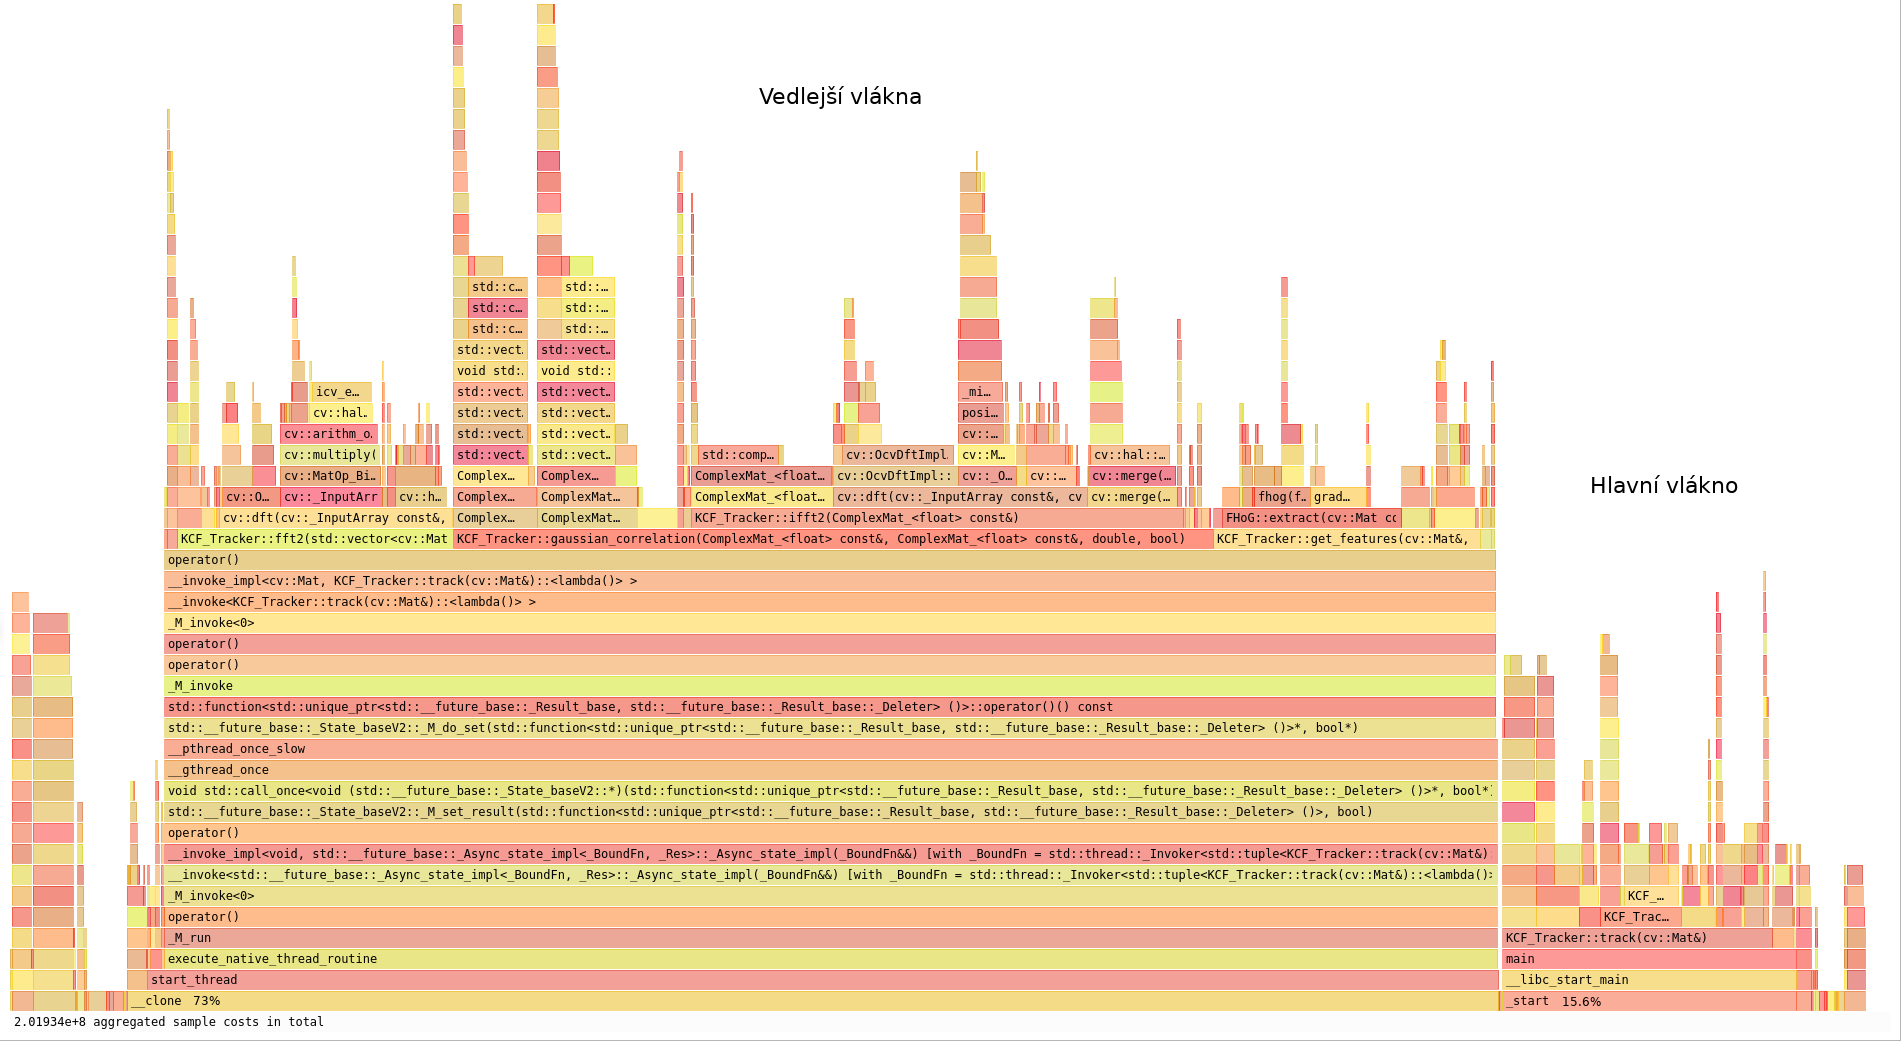
\includegraphics[width=\linewidth]{/home/shanigen/Pictures/Perf/Bag/LLC-References-bag-whole-gimp.png}
	\caption{LLC-References-bag}
	\label{LLC-References-bag-whole}
	\vspace{0.3cm}
	\centering
	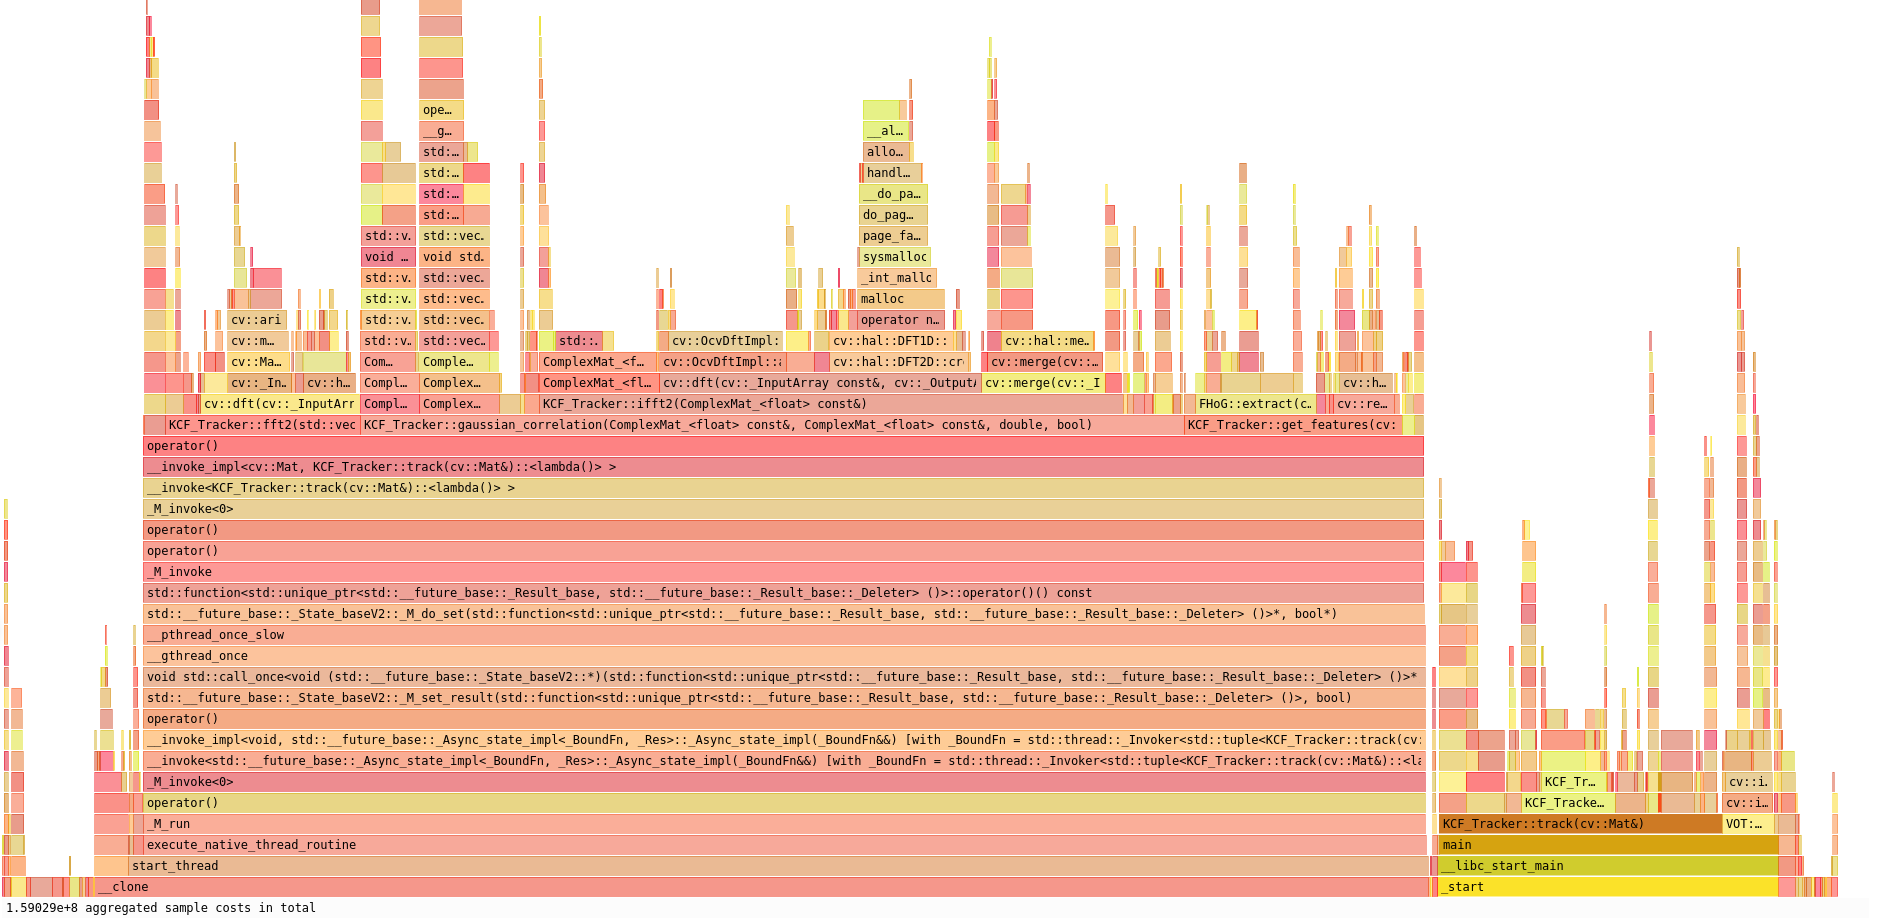
\includegraphics[width=\linewidth]{/home/shanigen/Pictures/Perf/car2/LLC-References-car2-whole.png}
	\caption{LLC-References-car2}
	\label{LLC-References-car2-whole}
\end{figure}
\begin{figure}[h!]
	\centering
	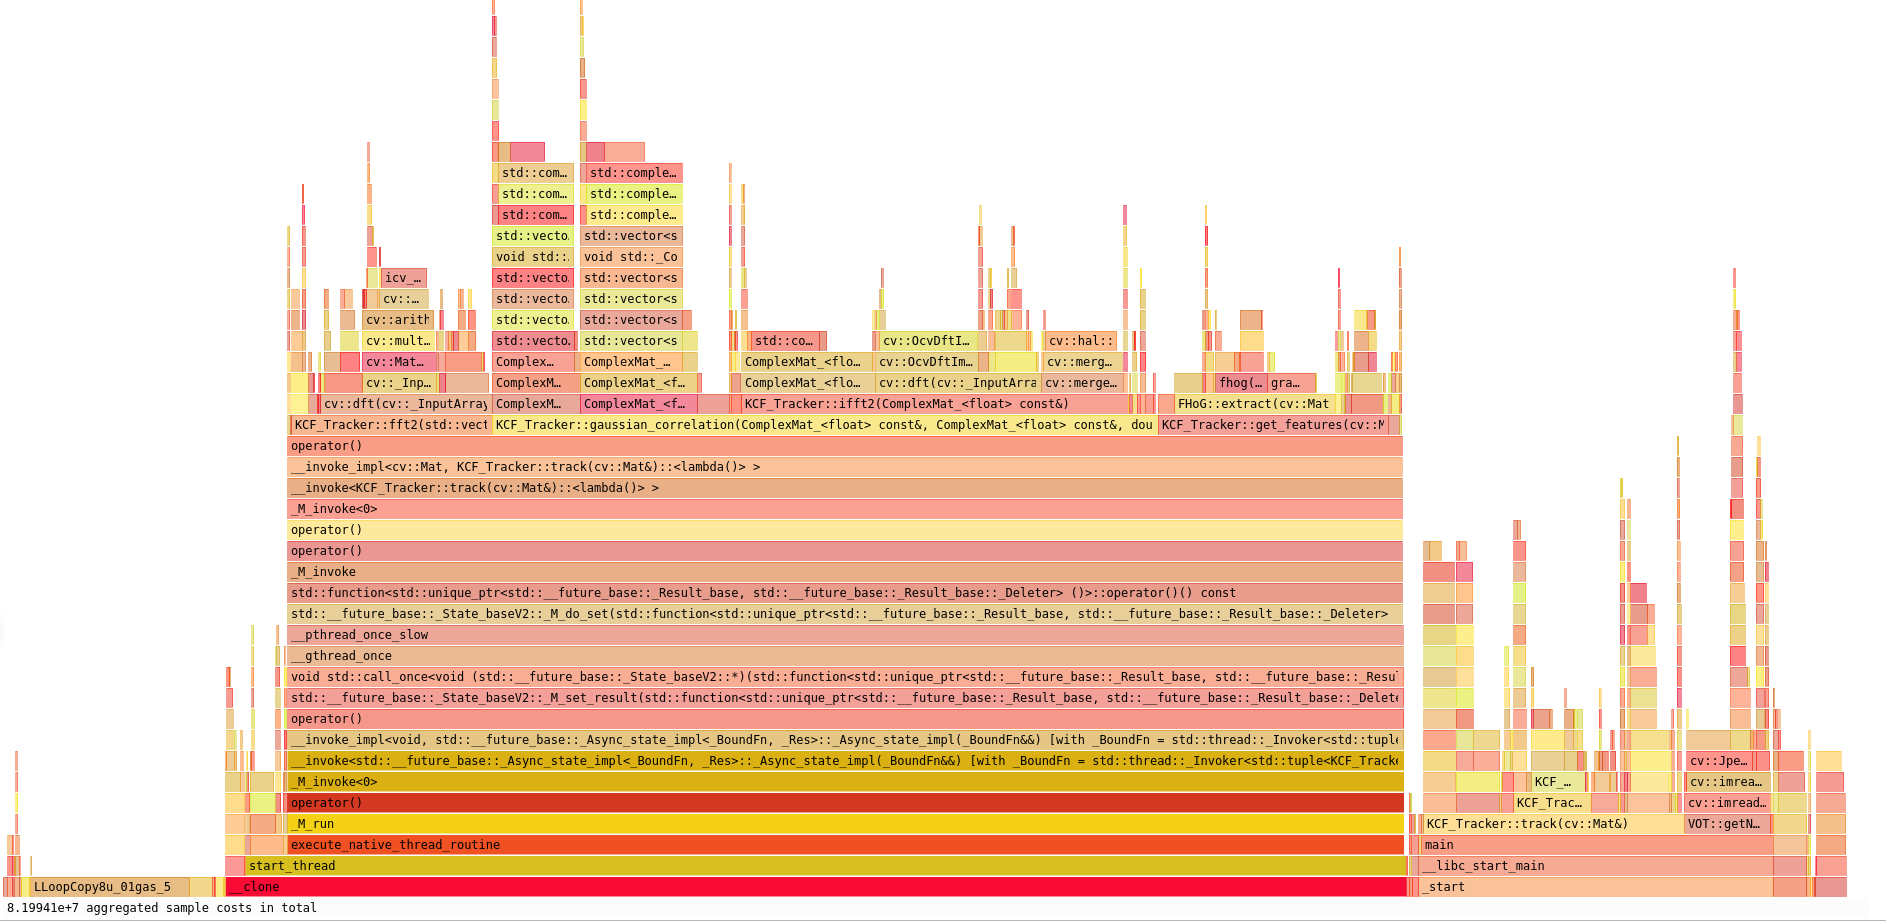
\includegraphics[width=\linewidth]{/home/shanigen/Pictures/Perf/ball1/LLC-References-ball1-whole.png}
	\caption{LLC-References-ball1}
	\label{LLC-References-ball1-whole}
\end{figure}
Na snímcích \ref{LLC-References-bag-whole}, \ref{LLC-References-car2-whole} a \ref{LLC-References-ball1-whole} jsou vidět výsledky z Perfu pro LLC-References. Každý z bloků ukazuje o jakou funkci se jedná a velikost znázorňuje kolik \% z celkového počtu zaznamenaných LLC-referencí se objevilo v dané funkci. Pokud ze sebe funkce volá další funkci objeví se jako blok v další úrovni, stejně tak i rekurze.\\
U všech datasetů lze vidět velmi podobné výsledky. U všech datasetů se většina LLC-Referencí vyskytovala ve vedlejších vláknech, která se vytvářejí v async časti track. Přesná čísla jsou v této tabulce:\\
\begin{center}
\begin{tabular}{|c|c|c|}
	\hline 
	& Vedeljší vlákna(\%) & Hlavní vlákno(\%) \\ 
	\hline 
	Bag & 73 & 15.6 \\ 
	\hline 
	Ball1 & 63.2 & 19 \\ 
	\hline 
	Car2 & 71.5 & 18.3 \\ 
	\hline
\end{tabular}
	\captionof{table}{Počet LLC-referencí vedlejsích vláken a hlavního vlákna v datasetech}
\end{center}
Do detailů jsou vedlejší vlákna a hlavní vlákno zobrazena na dalších snímcích. Všechny patří pod dataset bag, ostatní datasety nebyly do detailně zobrazeny, protože u všech se vyskytují stejné hotspoty(Místa ve kterých program tráví nejvíc času nebo místa, kde se nejvíce vyskytují sledované veličiny nejvíce,dále jen hotspot). Zvírazněny byly všechny funkce s počtem LLC referencí minimálně 1\% a u knihovních funkcí pouze ty,které byly voláné z programu a knihovní funkce voloné z kníhovních funkcí už ne.
\newpage
\paragraph{Hlavní vlákno}
Na obrázku \ref{LLC-References-main} je příbližení hlavního vlákna pro subset bag. Nejvíce LLC referencí se objevuje ve funkci track. Zde je hlavní hotspot gaussian\_correlation,která se používá i mimo async část, pak operátory z třídy ComplexMat, Fourierova transformace ve funkci fft2 a funkce get\_features. Většina zbylích LLC referencí je ve funkci getNextImage, která se stará o načítaní snímků. Zde patří z 1.08\%, 1.07\% LLC referencí knihovní funkci cv::imread.
\begin{figure}[h]
	\centering
	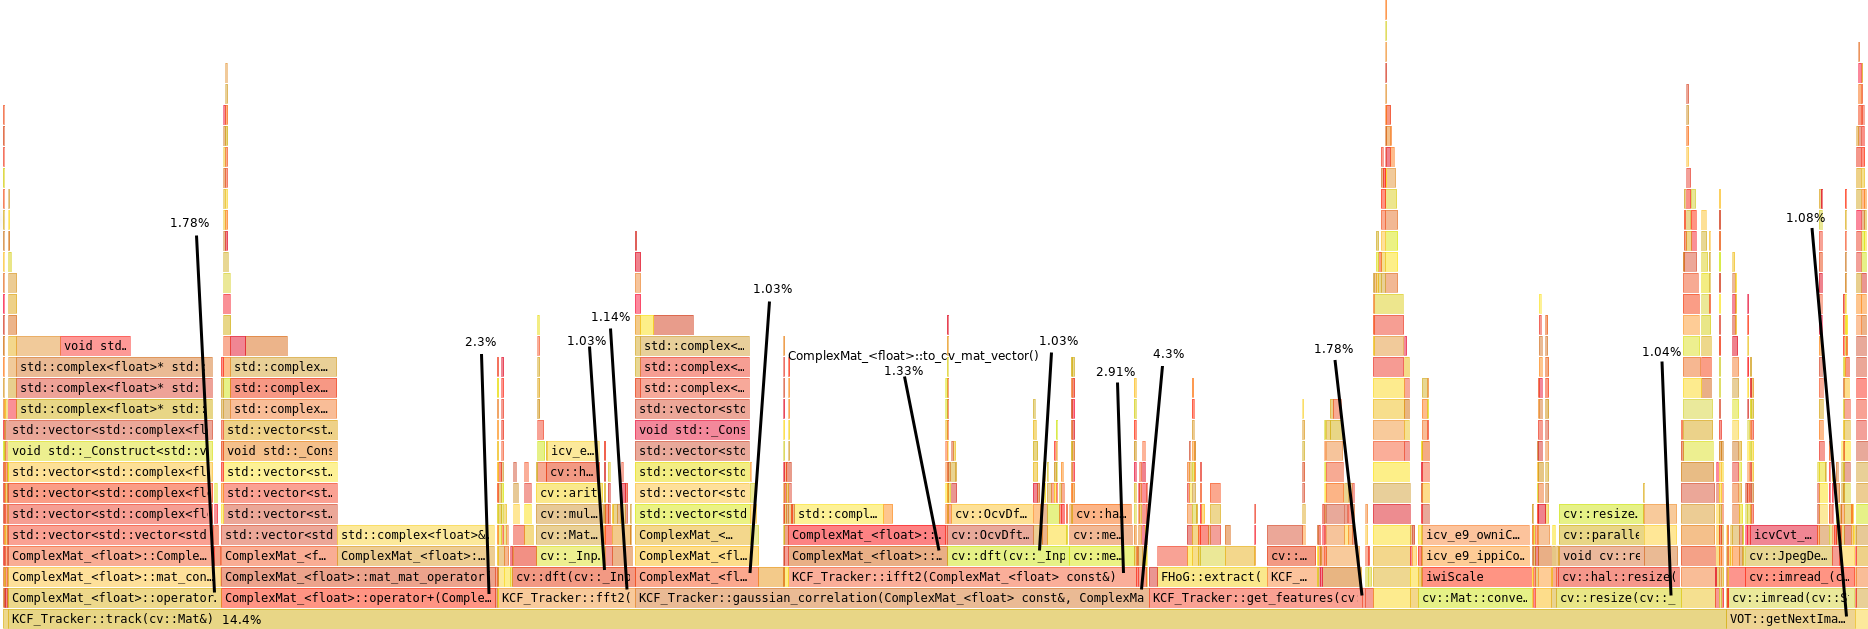
\includegraphics[width=\linewidth]{/home/shanigen/Pictures/Perf/Bag/LLC-References-bag-closeup-main-gimp.png}
	\caption{Hlavní vlákno-bag:LLC-Reference}
	\label{LLC-References-main}
\end{figure}
\paragraph{Vedlejší vlákna}
Stejně jako u hlavního vlákna lze vidět na obrázku \ref{LLC-References-threads} se většina LLC referencí u vedlejších vláken vyskytuje ve funkci gaussian\_correlation, kde je hotspot funkce ifft2. Další dva hotspoty jsou funkce get\_features a fft2. Na obrázku si lze všimnout, že oba výskyty knihovní funkce cv::dft v součtu dávají 25.9\% z celkového počtu LLC referencí pro celý program.
\begin{figure}[h!]
	\centering
	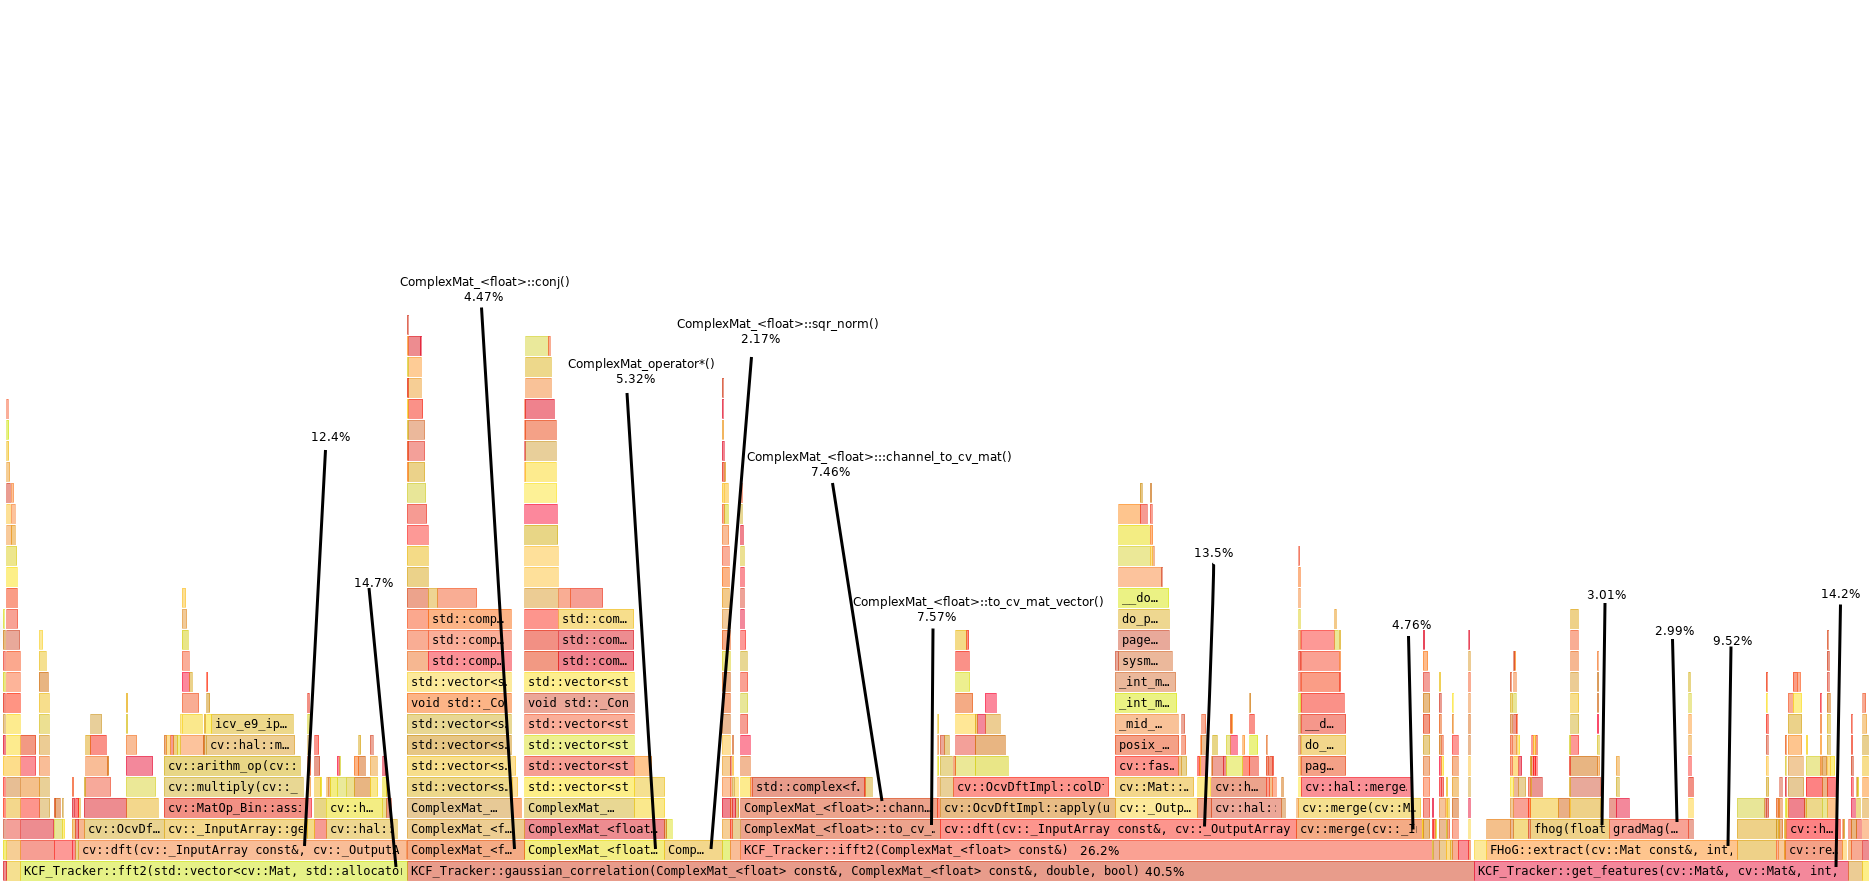
\includegraphics[width=\linewidth]{/home/shanigen/Pictures/Perf/Bag/LLC-References-bag-closeup-threads-gimp.png}
	\caption{Vedlejší vlákna-bag:LLC-Rereference}
	\label{LLC-References-threads}
\end{figure}
\newpage
\subsubsection{LLC Miss}
\begin{figure}[h!]
	\centering
	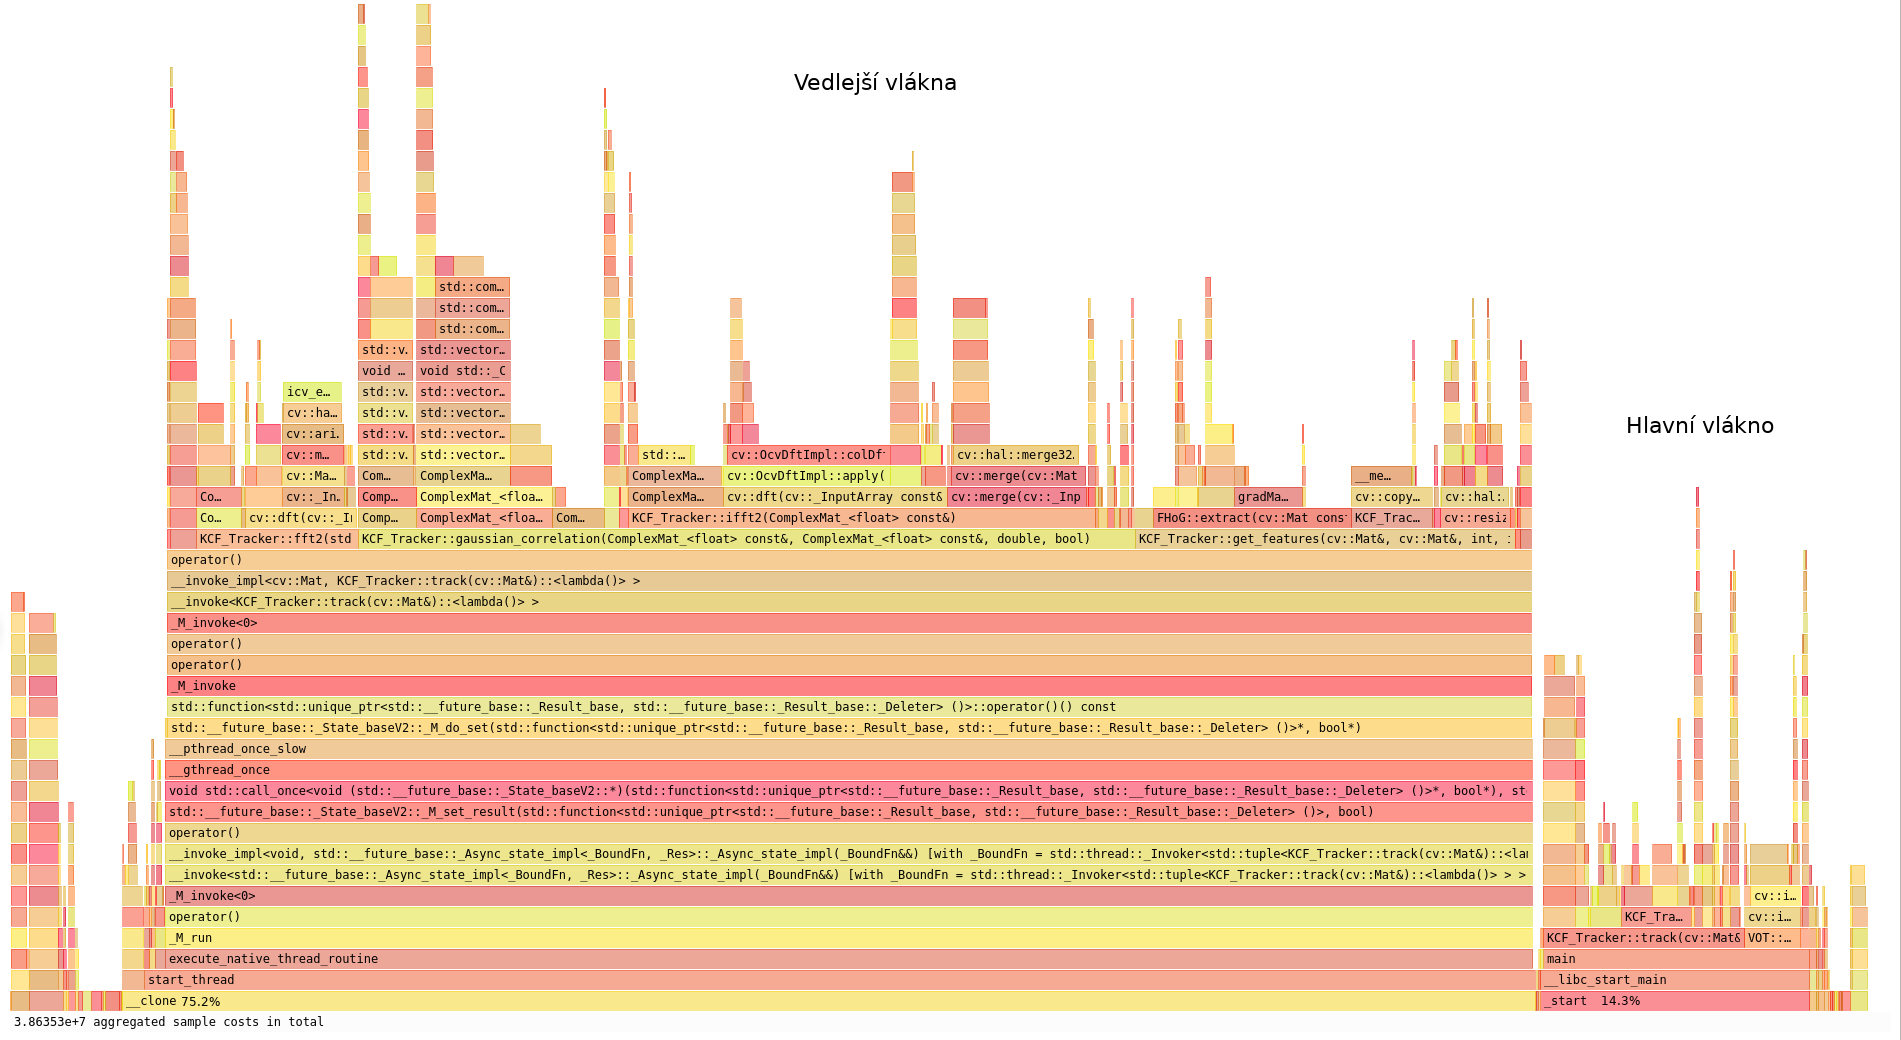
\includegraphics[width=\linewidth]{/home/shanigen/Pictures/Perf/Bag/LLC-Miss-bag-whole-gimp.png}
	\caption{LLC-Miss-bag}
	\label{LLC-Miss-bag-whole}
	\vspace{0.3cm}
	\centering
	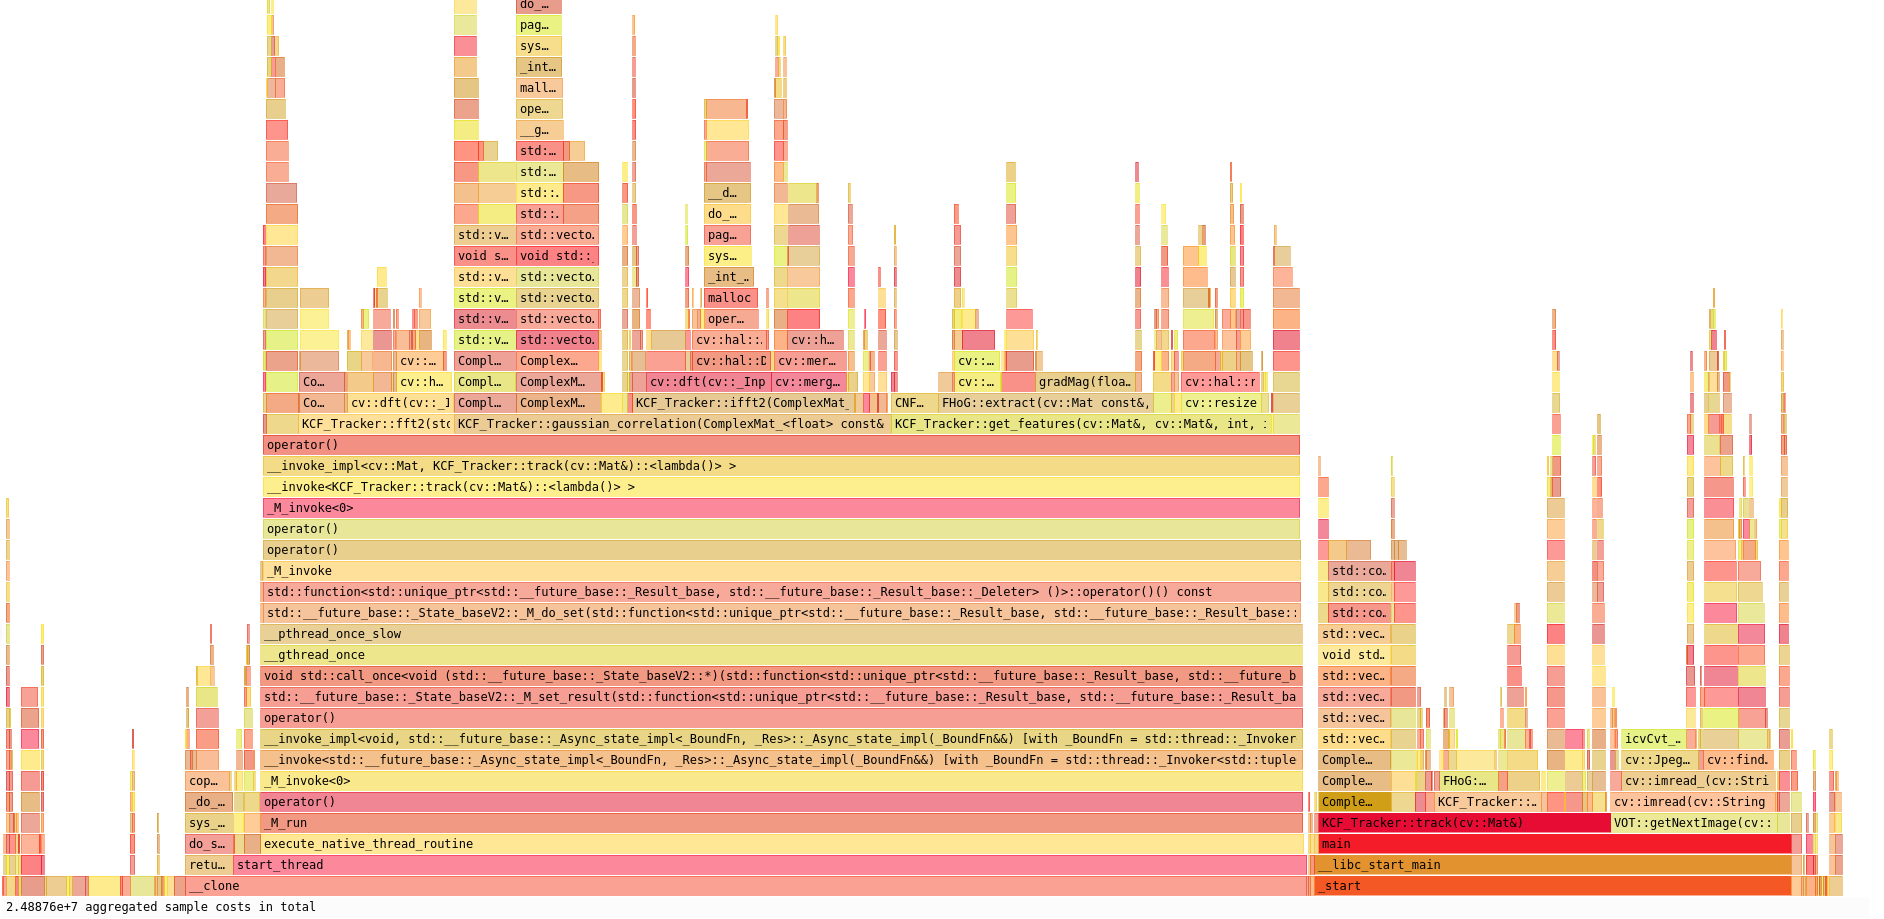
\includegraphics[width=\linewidth]{/home/shanigen/Pictures/Perf/car2/LLC-Misses-car2-whole.png}
	\caption{LLC-Miss-car2}
	\label{LLC-Miss-car2-whole}
\end{figure}
\newpage
\begin{figure}[h!]
	\centering
	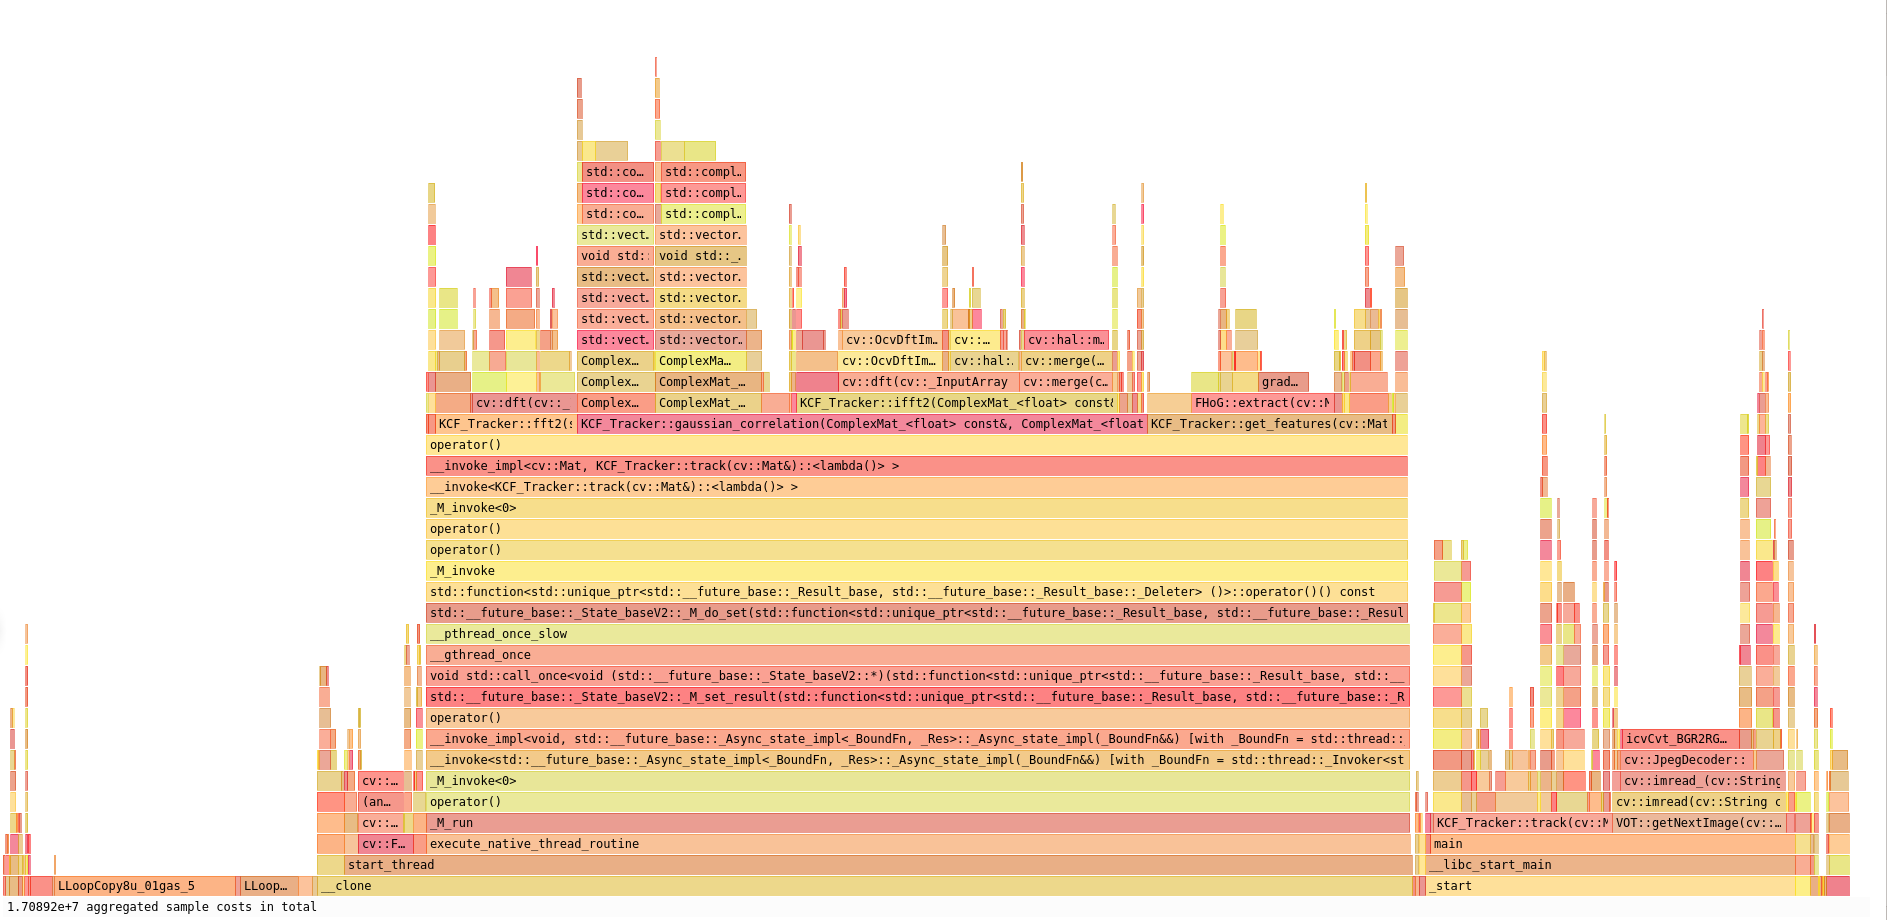
\includegraphics[width=\linewidth]{/home/shanigen/Pictures/Perf/ball1/LLC-Misses-ball1-whole.png}
	\caption{LLC-Miss-ball1}
	\label{LLC-Miss-ball1-whole}
\end{figure}
Na snímcích \ref{LLC-Miss-bag-whole}, \ref{LLC-Miss-car2-whole} a \ref{LLC-Miss-ball1-whole} lze vidět, že výskyt LLC missů se objevuje především ve vedlejších vláknech. Přesná čísla pro všechny datasety jsou v této tabulce:
\begin{center}
	\begin{tabular}{|c|c|c|}
		\hline 
		& Vedeljší vlákna(\%) & Hlavní vlákno(\%) \\ 
		\hline 
		Bag & 75.2 & 14.3 \\ 
		\hline 
		Ball1 & 58.7 & 19.8 \\ 
		\hline 
		Car2 & 60.1 & 25.5 \\ 
		\hline
	\end{tabular}
	\captionof{table}{Počet LLC-missů vedlejsích vláken a hlavního vlákna v datasetech}
\end{center}
Stejně jako u LLC referencí jsou na dalších snímcích detailně zobrazena vedlejší vlákna a hlavní vlákno pro dataset bag.
\newpage
\paragraph{Hlavní vlákno}
Přestože nejvíce LLC referencí má v hlavním vlákně ve funkci track funkce gaussian\_correaltion, jak bylo vidět na snímku \ref{LLC-References-main}, tak na obrázku \ref{LLC-Miss-main} se nejvíce LLC missů objevuje ve funkci get\_features. V ní hlavně u funkcí FHoG::extract(Def:line 20,fhog.hpp,dále jen extract) a KCF\_Tracker::
get\_subwindow(Def:line 491,kcf.cpp,dále jen get\_subwindow). Mimo funkci track se vyskytly LLC missy především při načítání snímků ve funkci getNextImage.
\begin{figure}[h!]
	\centering
	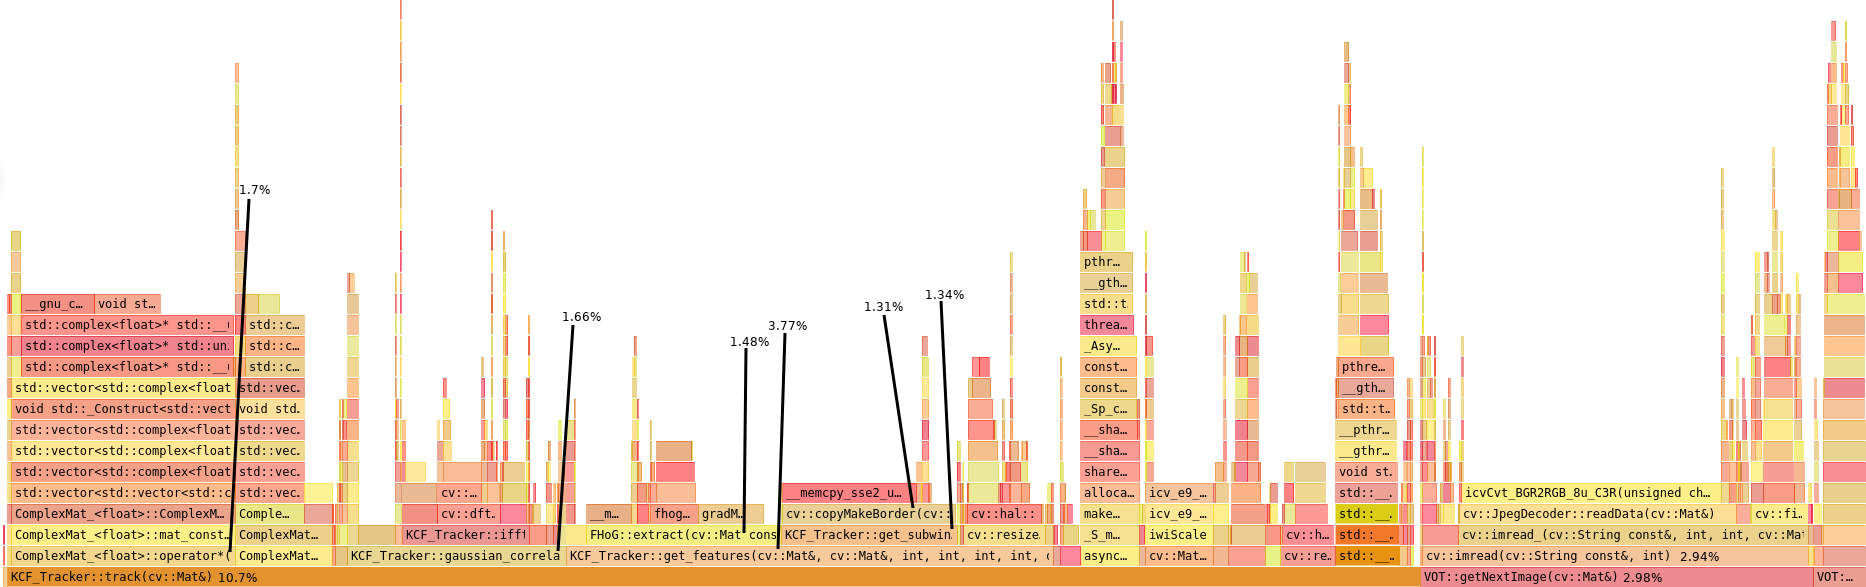
\includegraphics[width=\linewidth]{/home/shanigen/Pictures/Perf/Bag/LLC-Miss-bag-closeup-main-gimp.png}
	\caption{Hlavní vlákno-bag:LLC-Miss}
	\label{LLC-Miss-main}
\end{figure}
\paragraph{Vedlejší vlákna}
U vedlejších vláken se 41.4\% všech LLC missů z celého programu vyskytuje ve funkci gaussian\_correlation, která je volaná v async cásti. V ní víc jak polovina všech LLC missů je ve funkci ifft2, kde se provádí Fourierova transformace. Vedle gaussian\_correlation je dalším hotspotem znovu funkce get\_features, stejně jako v hlavním vlákně. Funkce get\_features dohromady s funkcí ifft2 davají v součtu 45.1\% všech LLC missů.
\begin{figure}[h!]
	\centering
	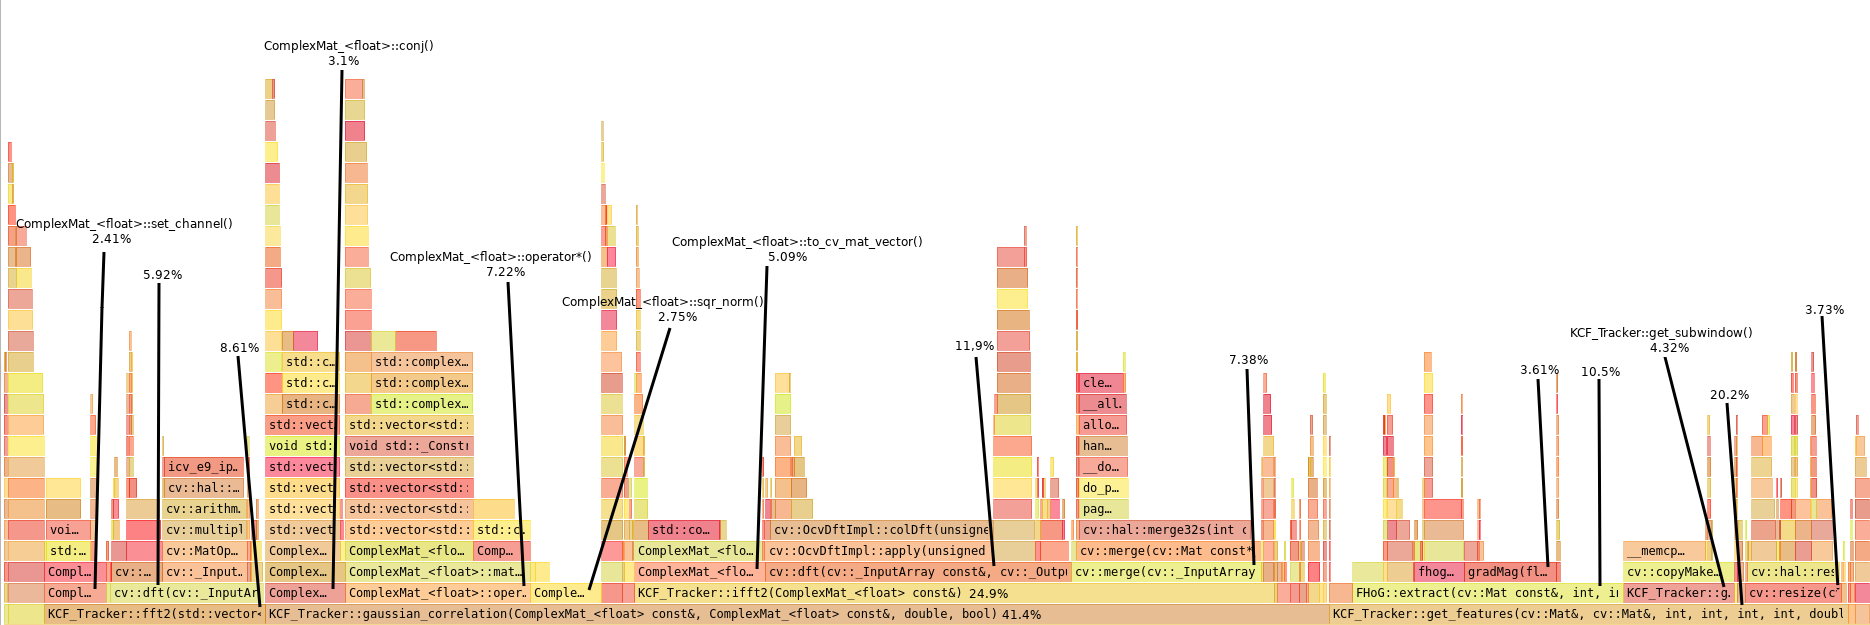
\includegraphics[width=\linewidth]{/home/shanigen/Pictures/Perf/Bag/LLC-Miss-bag-closeup-threads-gimp.png}
	\caption{Vedlejší vlákna-bag:LLC-Miss}
	\label{LLC-Miss-threads}
\end{figure}
\newpage
\subsection{Intel® VTune™ Amplifier XE 2017 Update 4}
Analýza proběhla pouze na datasetu bag. Na obrázku \ref{Amp-summary} je vidět jaký druh Hardware eventů byl měřen i celkový počet zaznamenaných eventů. Amplifier oproti Perfu má mhohem menší počet záznamů, a proto i celkový počet LLC-missů a LLC-Hitů je mnohem menší.
\begin{figure}[h!]
	\centering
	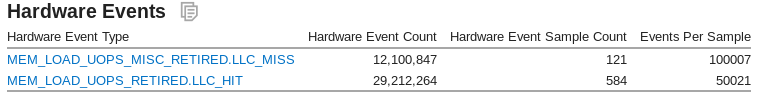
\includegraphics[width=\linewidth]{/home/shanigen/Pictures/Amplifier/Bag/Summary-bag.png}
	\caption{Souhrn analýzy}
	\label{Amp-summary}
\end{figure}
\\
Na obrázku \ref{Amp-detail} je detailnější výsledek analýzy seřazen sestupně podle LLC-Missů. Červeným puntíkem jsou označeny funkce z OpenCV a KCF trackeru, ke kterým se mi podařilo najít informace o užití a funkci. Vyjímkou je funkce cv::utils::trace::details::parallelForFinalize (Def:line 962,trace.cpp,dále jen parallelForFinalize). Ke které se mi nepodařilo najít zádne informace v dokumentaci ani fórech OpenCV.
\begin{figure}[h!]
	\centering
	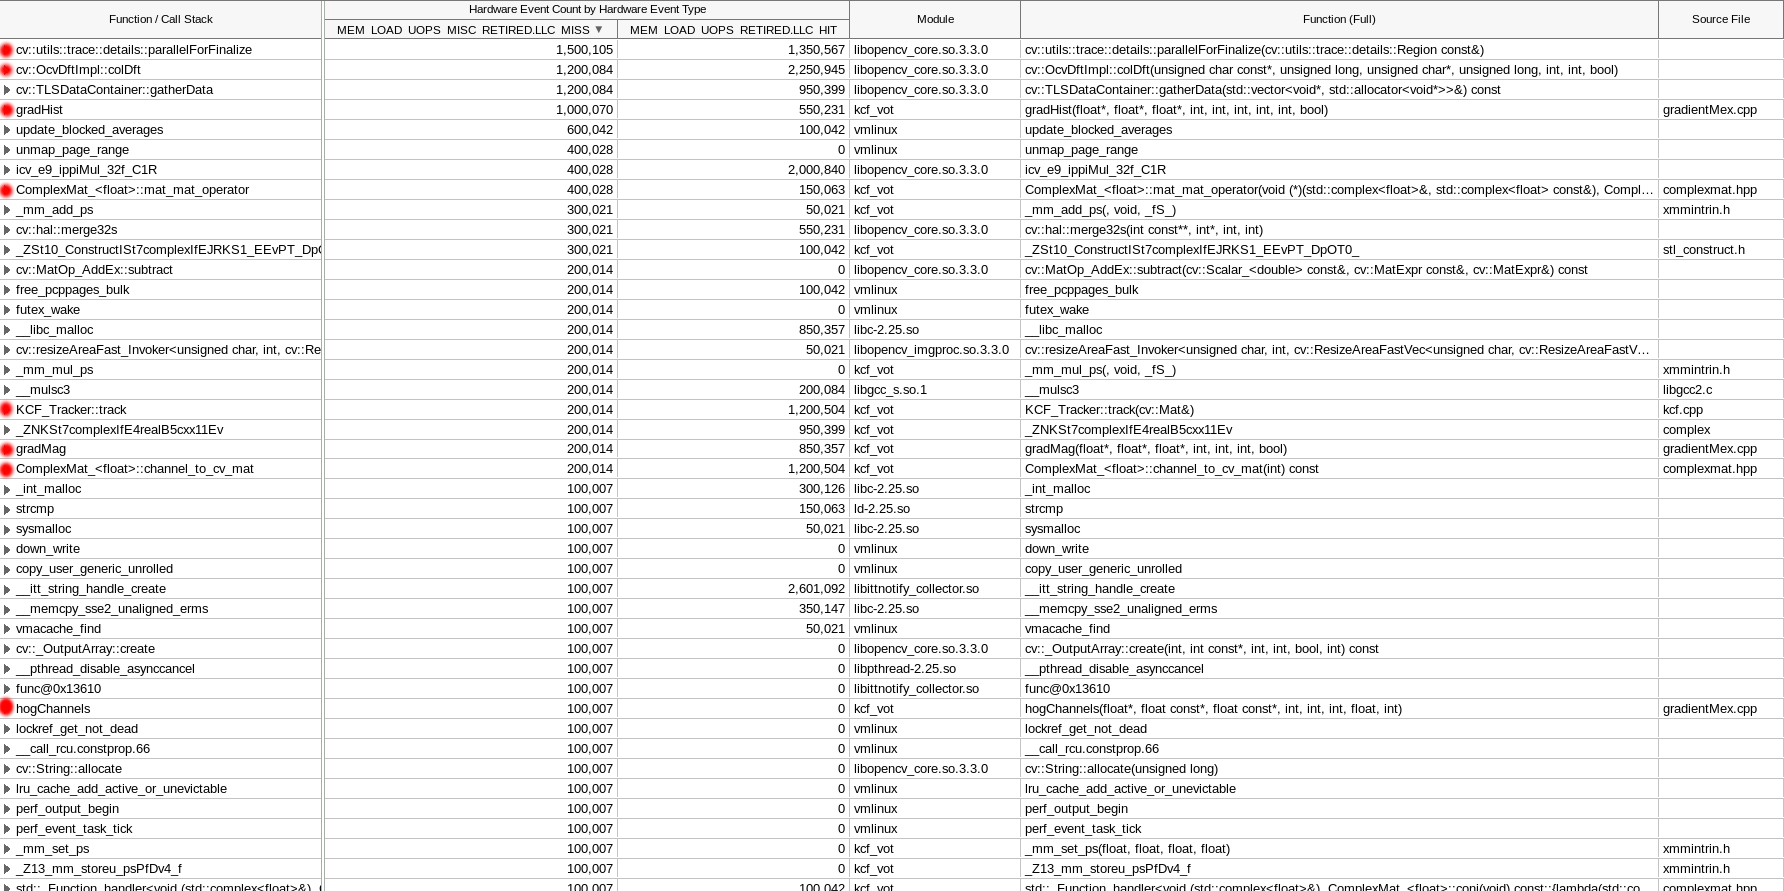
\includegraphics[width=\linewidth]{/home/shanigen/Pictures/Amplifier/Bag/Detail-bag-gimp.png}
	\caption{Detailní výsledek analýzy}
	\label{Amp-detail}
\end{figure}
\\
Nejvíce LLC missů amplifier zaznamenal ve funkci cv::utils::trace::details::
parallelForFinalize (Def:line 962,trace.cpp, dále jen parallelForFinalize). Perf tuto funkci nezaznamenal místo ní zaznamenal funkci cv::parallel\_for\_(Def:line 372,parallel.cpp, dále jen parallel\_for\_), která slouží podle dokumentací a fór OpenCV k paralelizaci funkcí v OpenCV. Parallel\_for\_ se používá ve funkc cv::resize, která se vyskytuje ve funkci get\_features. Ampliefier tuto funkci zase naopak nezaznamenal vůbec. Funkce cv::OcvDftImpl::colDft(Def:line 2923,dxt.cpp, dále jen colDft) se využívá v cv::dft, která se používá jak v ifft2, tak i v fft2. Ifft2 se navíc ještě vyskytuje i v gaussian\_correlation. Tuto funkci Perf také nezaznamenal. ComplexMat\_<float>::mat\_mat\_operator(Def:line 147,complexmat.hpp), která se využívá v přetěžování operátorů v třídě ComplexMat\_. GradHist(Def:line 148, gradientMex.cpp) spolu s hogChannels(Def:line 256,gradientMex.cpp) se využívá při výpočtu HoG(Histogram Of oriented Gradient \url{https://en.wikipedia.org/wiki/Histogram_of_oriented_gradients}) ve funkci fhog(Def:line 298,gradientMex.cpp), která se náchazí v extract, kde se vyskytuje i funkce gradMag(Def:line 59, gradientMex.cpp), která slouží k výpočtu velikosti a orientace gradientu ve všech místech obrázku. Track, jak už bylo zmíněno v popisu programu, je hlavní funkce programu a probíha v ní hlávní část výpočtů tak obsahuje i async část.  ComplexMat\_<float>::channel\_to\_cv\_mat(Def:line 184,complexmat.hpp) slouží k získání realné a imaginární složky komplexních výsledků pří diskrétní Fourierově transformaci.
\subsection{Porovnání výsledků}
Výsledky z Perfu a Amplifieru nebyly úplně stejné. Největším rozdílem byla především funkce parallelForFinalize, která měla nejvíce LLC missů v Amplifieru, a kterou Perf vůbec nezaznamenal při profilování. Navíc online není k této funkci dostatek informací od OpenCV a funkce colDft, kterou také zaznamenal pouze Amplifier. U Amplifieru se navíc stejný počet LLC missů a hitů objevil u několika funkcí. Intel má optimalizované analýzy na své architektury procesorů, což může ovlivňovat výsledky stejně tak i to, že Intel přímo nepodporuje Arch linux, na kterém proběhlo profilovní. S Perfem se však ve funkcích get\_features a přetížené operátory v třídě ComplexMat\_ výsledky podobají. Obě patří mezi funkce s nejvíce LLC-Missy.
\end{document}